\begin{beamercolorbox}[center,wd=\textwidth]{postercolumn}
        \begin{minipage}[T]{.95\textwidth}  % tweaks the width, makes a new \textwidth
          \parbox[t][\columnheight]{\textwidth}{ % must be some better way to set the the height, width and textwidth simultaneously
            % Since all columns are the same length, it is all nice and tidy.  You have to get the height empirically
            % ---------------------------------------------------------%
            % fill each column with content            
            \begin{block}{1. Introduction}
              \begin{itemize}
              \item Frontier-based exploration is the most common approach
              to exploration
              \item \emph{Frontier}: a segment that separates known regions
                from unknown regions
                \begin{itemize}
                \item Frontier is a set of points
                \item Each point has at least one \emph{open-space} neighbor
                \end{itemize}
              \item By moving towards frontiers, robot keeps discovering new
              regions
              \item We present two novel frontier detection algorithms:
                \begin{itemize}
                \item \emph{WFD}, a graph search based algorithm
                \item \emph{FFD}, based on processing only the new laser
                readings data
                \end{itemize}
              \end{itemize}              
            \end{block}
            \vfill
            
            \begin{block}{2. Existing Frontier Detection is Slow}

              \begin{itemize}
                  \item Frontier detection algorithms rely on computer vision
                  methods
                    \begin{itemize}
                    \item Edge-detection and region extraction
                    \end{itemize}
                  \item They have to process the entire map data with every
                  execution
                  
                
                
                
	              \item Existing frontier detection algorithms take $\sim$10-30
	              seconds to run
	                    \begin{itemize}
	                    \item Even on powerful computers
	                    \item Exploring a large area forces the robot to wait in its
	                    spot
	                    \item Frontier detection is called \emph{only} when the
	                    robot arrives at its target
	                    \end{itemize}
	               \item Real-time frontier detection can shorten the exploration
	               time
		               \begin{itemize}
		                 \item Enables the robot to detect the relevance of its target
		                 in real-time
		               \end{itemize}
		               \begin{tabularx}{\linewidth}{ZZZ}
                    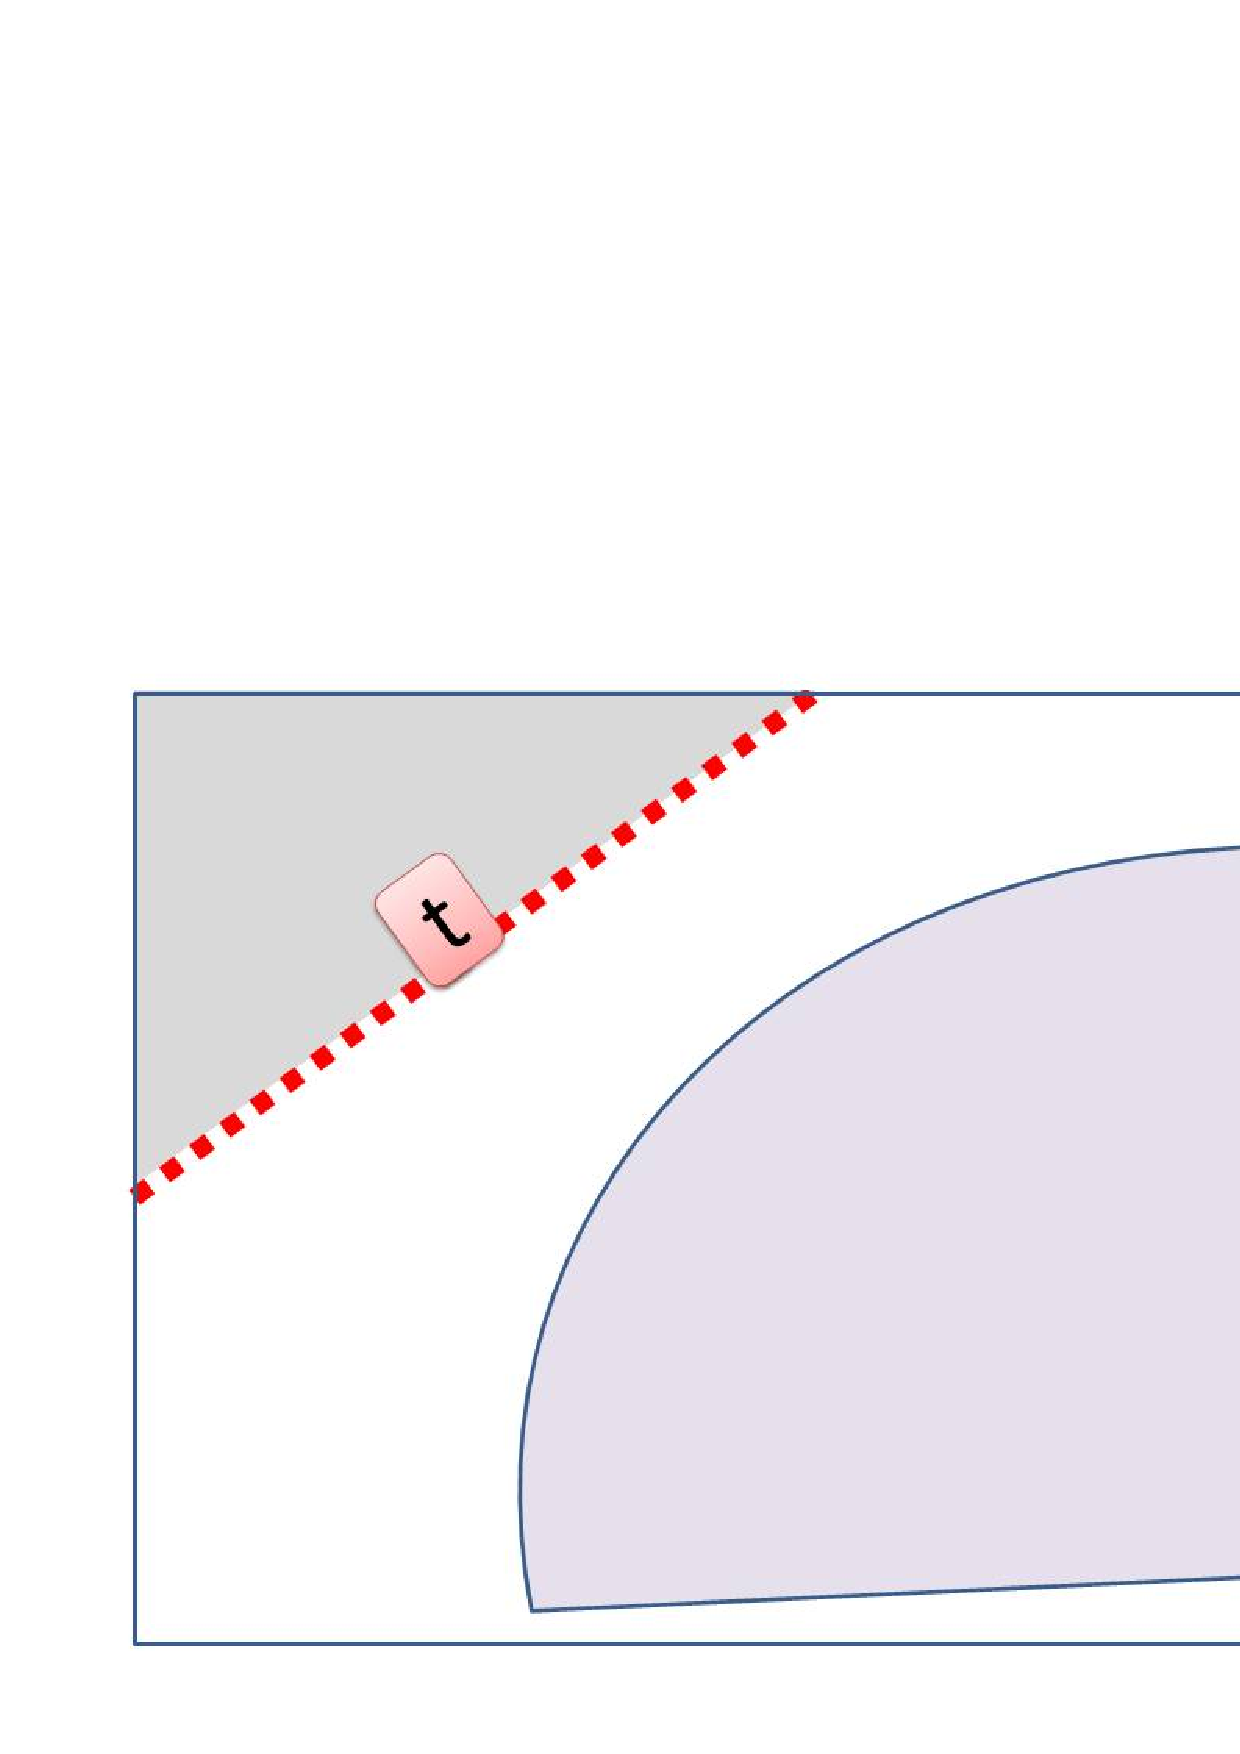
\includegraphics[width=0.7\linewidth]{images/single_1.JPG}
                    &
                    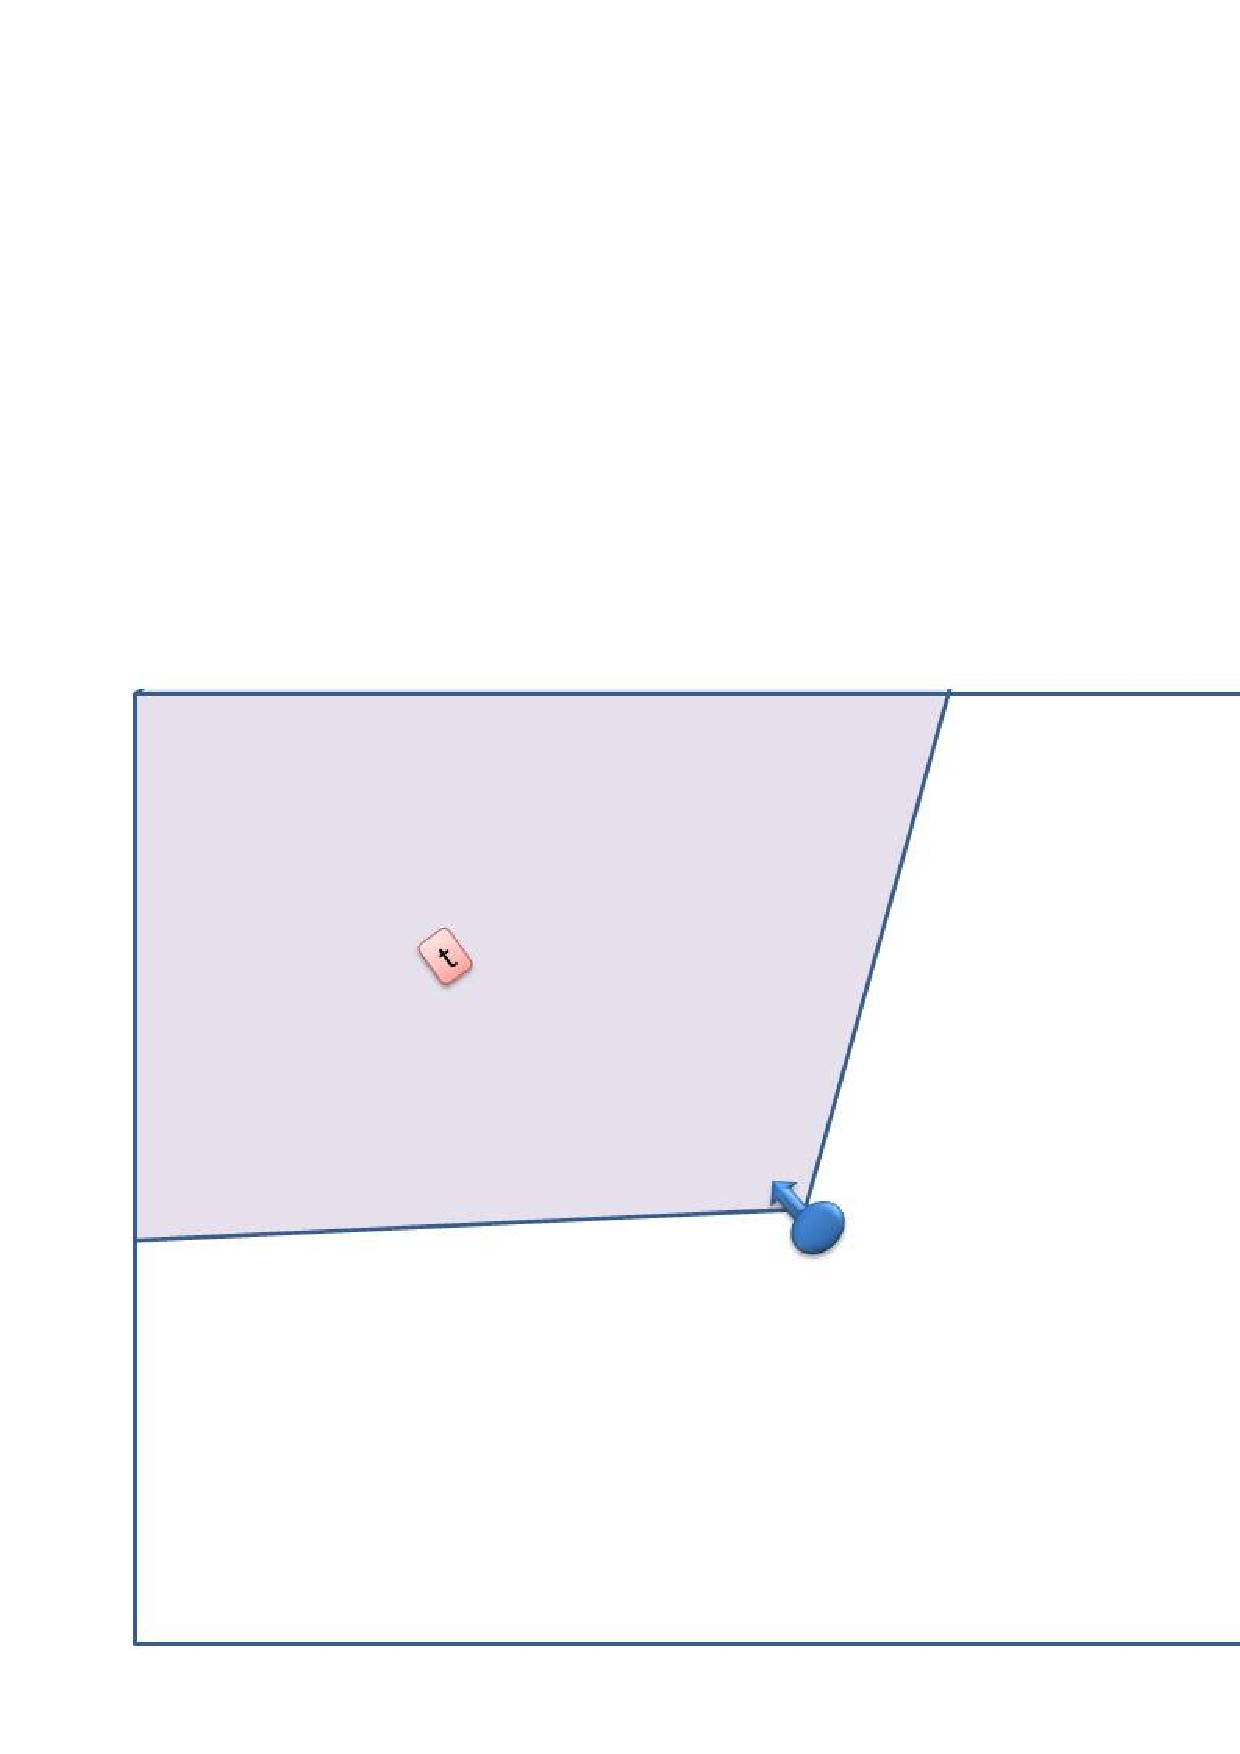
\includegraphics[width=0.7\linewidth]{images/single_2.JPG}
                    &
                    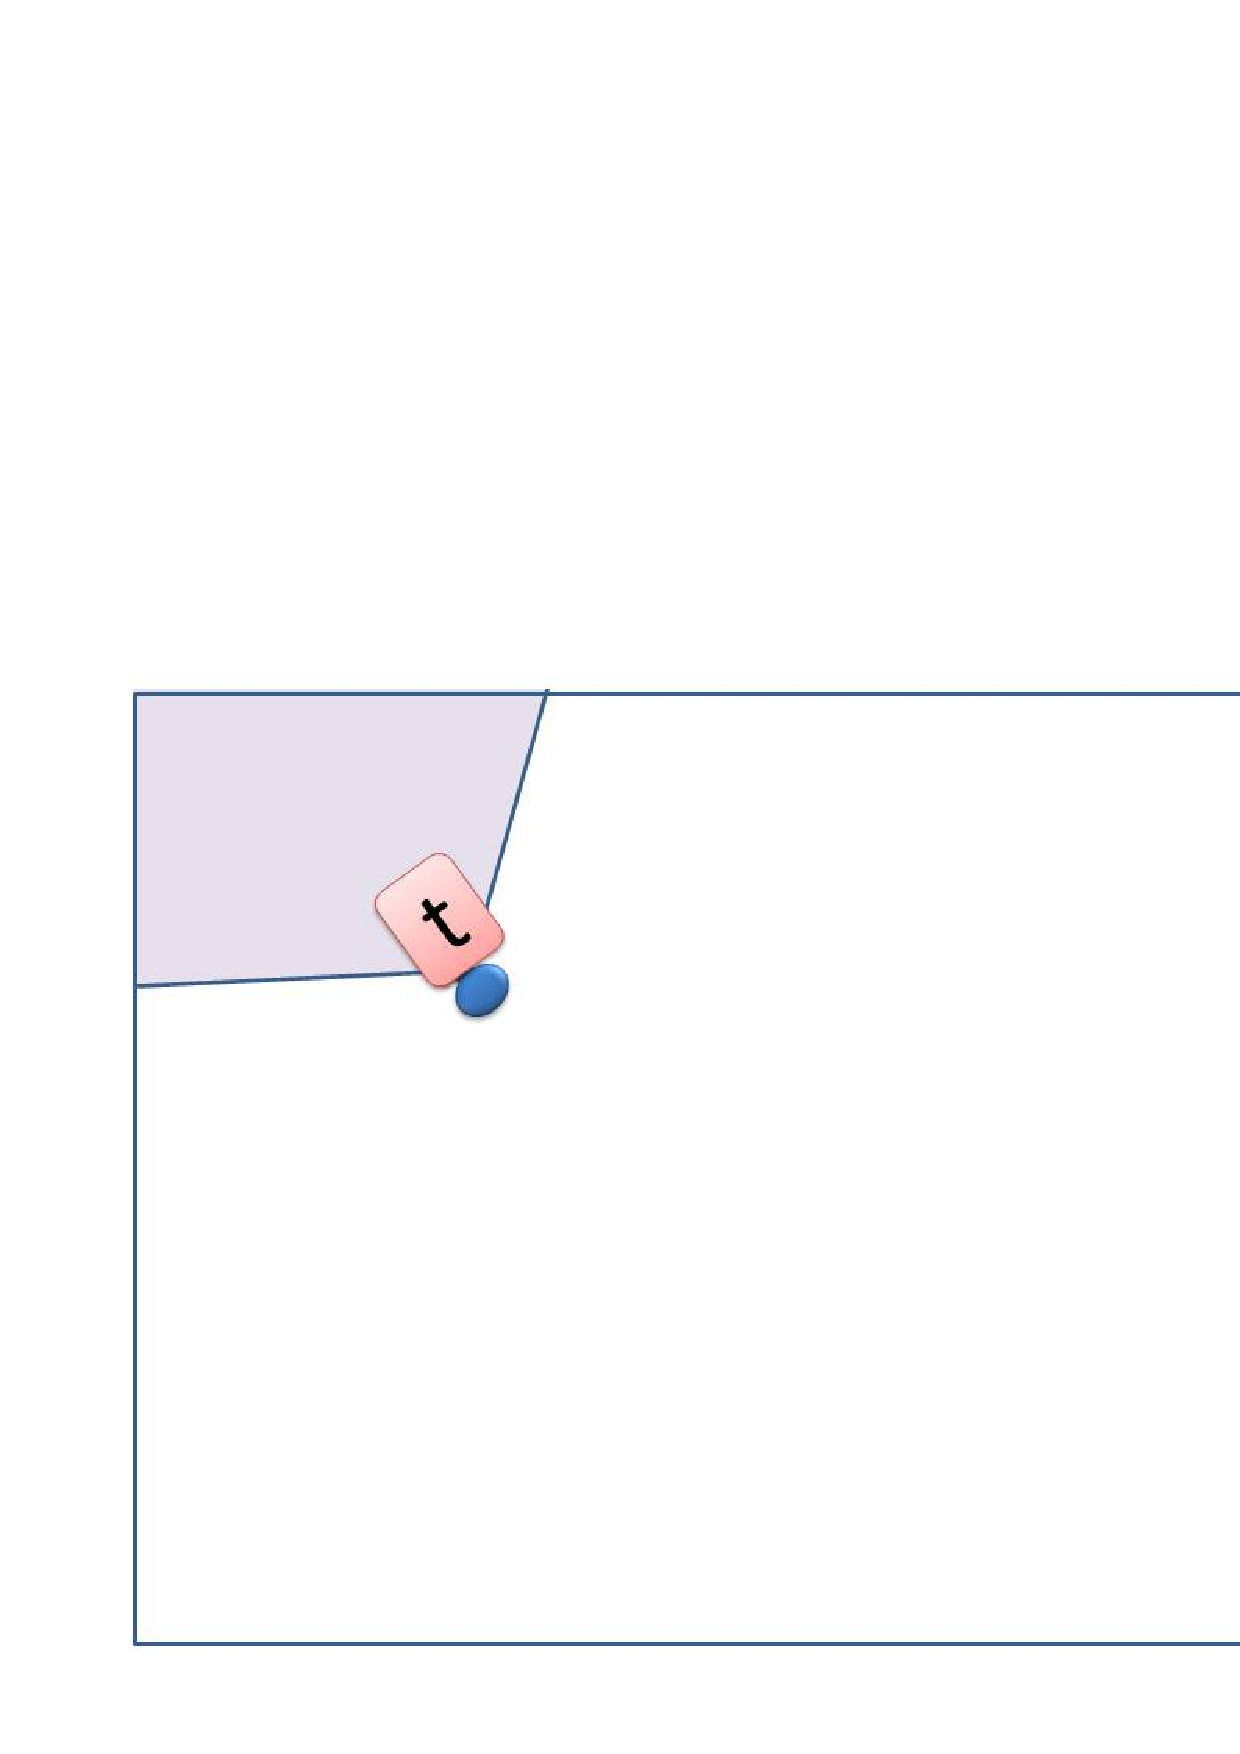
\includegraphics[width=0.7\linewidth]{images/single_3.JPG}
                  \end{tabularx}
              \end{itemize}
              \vskip-1ex
            \end{block}
            \vfill
            
            \begin{block}{3. WFD: Wavefront Frontier Detection}
              \begin{itemize}
              \item Breadth-first search for frontier detection
              \item \emph{WFD} avoids searching unknown regions
              \item \emph{WFD} scans only known regions
              \end{itemize}
            \end{block}
            \vfill
            
            \begin{block}{4. FFD: Fast Frontier Detection}
              \begin{itemize}
              \item Observation: scanning all known regions is unnecessary

                %\item descriptor vectors extracted at keypoints in a test image
                %$X$ are compared to all descriptor vectors extracted at
                %keypoints from the reference images $Y_n, n=1,\cdots,N$ by the
                %Euclidean distance
                %\item decision rule:
                %  \begin{align*}
                %    X \rightarrow r(X) & = \arg \max_{c} \Big\{ \max_n \big\{
                %    \sum_{x_i \in X} \delta(x_i,Y_{n,c})\big\} \Big\}
                %  \end{align*}
                %\item additionally, a ratio constraint is applied in
                %$\delta(x_i,Y_{n,c})$
                
              \item \emph{FFD} avoids searching both known and unknown regions
              \item \emph{FFD} consists of the following stages:
                \begin{itemize}
                \item (4.1) Sorting stage
                \item (4.2) Calculating contour stage 
                \item (4.3) Detecting new frontiers stage
                \item (4.4) Maintaining previously detected frontiers stage
                \end{itemize}

              \end{itemize}
            \end{block}
            \vfill
            
            \begin{block}{4.1 Sorting}
              \begin{figure}
%                \footnotesize
                %\centering
                  \includegraphics[width=0.88\linewidth]{images/sorting_arrows_png}
%                 \begin{tabular}{p{.20\linewidth}  p{.20\linewidth} 
%                 p{.20\linewidth}  p{.20\linewidth}}
% sorting_arrows_png
%                   \includegraphics[width=1.0\linewidth]{images/sorting_1.JPG}
%                   &
%                   \includegraphics[width=1.0\linewidth]{images/sorting_2.JPG}
%                   &
%                   \includegraphics[width=1.0\linewidth]{images/sorting_3.JPG}
%                   &
%                   \includegraphics[width=1.0\linewidth]{images/sorting_full_points.JPG}
%                 \end{tabular}
              \end{figure}
              \begin{itemize}
              \item Most laser sensors return readings that are already sorted
                \begin{itemize}
                \item Points that are sorted according to polar angle
                \item The robot as center
                \end{itemize}
              \item However, if it is not the case, we can sort them efficiently
					\begin{itemize}
					  \item by using \emph{cross-product}
					  \item $(p_1-p_0)\times(p_2-p_0)=(x_1-x_0)\cdot(y_2-y_0)-
					  (x_2-x_0)\cdot(y_1-y_0)$
					\end{itemize} 
              \end{itemize}
            \end{block}
            
            \vfill
            \begin{block}{4.2 Contour}
              \begin{figure}
%                \footnotesize
                %\centering
                \begin{tabular}{p{.30\linewidth}  p{.30\linewidth} 
                p{.30\linewidth} }

				  \raggedleft
                  \includegraphics[width=0.87\linewidth]{images/contour_vectors.JPG}
                  &
                  %\center{\huge{$ \to$ }}
                   			%\begin{textblock}{1}(0,-1) % relative x,y offsets from current position 
		          
		          \pgfbox[center,center]{ 
		            \begin{tikzpicture}[overlay,line width = 0.5cm, blue] 
		              \draw[->] (2,3) -- (11.5,3); 
		            \end{tikzpicture} 
		          } 
                  &
                  \includegraphics[width=0.87\linewidth]{images/contour.JPG}
                \end{tabular}
              \end{figure}
              \vspace{-50pt}
              \begin{itemize}
              \item \textbf{Input}: sorted set of points
              \item \textbf{Output}: a contour that is built from the laser
              readings set
                \begin{itemize}
                \item The line that connects each two adjacent points from the
                set
                \end{itemize}
              \item Calculate the points that lie between each adjacent laser
              readings
              \item We need the algorithm to be fast and robust against rounding
              errors
					\begin{itemize}
					  \item We use \emph{Bresenham's line algorithm} [Bresenham (1965)]
					\end{itemize} 
              \end{itemize}
            \end{block}
          }
        \end{minipage}
      \end{beamercolorbox}